\section{Aufbau und Durchführung}
\label{sec:Durchführung}

  \subsection{Aufbau}

  Der Versuchsaufbau ist in Abbildung \ref{fig:aufbau} dargestellt.
  Eine Rubidiumspektrallampe emitiert Licht, welches durch eine Sammellinse kollimiert wird.
  Ein Interferenzfilter lässt nur die $D_1$-Linie durch, das Licht wird danach von einem Polarisator zunächst linear polarisiert, um danach durch ein $\lambda/4$-Plättchen rechtszirkular polarisiert zu werden und auf die Dampfzelle zu scheinen. Diese wird beheizt und ist mit einem Gasgemisch aus Rubidium und Neon-Puffergas gefüllt, welches verhindert, dass die Besetzungsinversion durch Stöße des Rubidiums mit den Wänden der Dampfzelle abgeschwächt oder verhindert wird. Stöße zwischen den Rubidium- und Neonatome können keinen Drehimpuls zwischen den Elektronenhüllen austauschen, sodass das Herstellen der Besetzungsinversion dadurch nicht behindert wird. Hinter der Dampfzelle wird das Licht auf eine Photozelle fokussiert, wodurch die Transparenz des Gases für die $D_1$-Linie gemessen wird. Das Signal wird dabei auf den Y-Eingang eines Oszilloskop gegeben.

  \begin{figure}
    \centering
    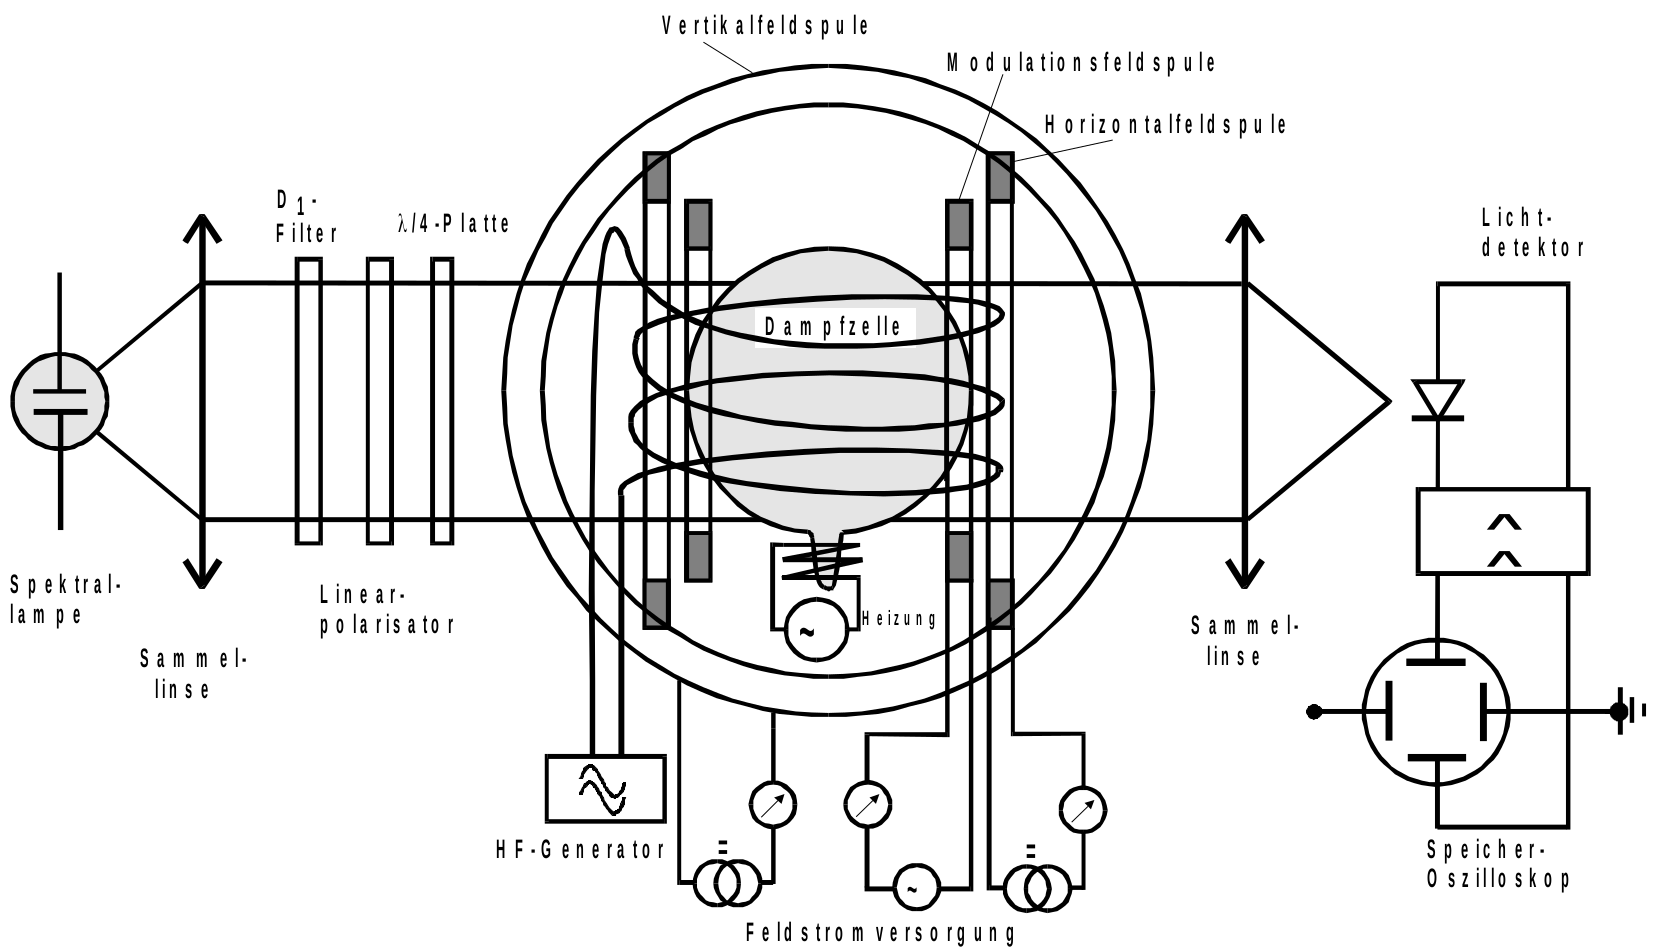
\includegraphics[width=\textwidth]{pictures/aufbau.png}
    \caption{insert description \cite{stehendeWelle}.}
    \label{fig:aufbau}
  \end{figure}

  Es stehen drei Helmholtzspulen zur Verfügung, um Magnetfelder anzulegen. Eine Horizontalfeldspule erzeugt ein statisches Horizontalfeld, während die Sweep-Spule auf die Horizontalfeldspule aufgewickelt ist und ein Sägezahnsignal liefert. Das RF-Feld wird mit einem externen Funktionsgenerator angesteuert.

  \subsection{Durchführung}

  Zu Beginn des Versuchs wird der Strahlengang auf eine maximale Intensität eingestellt und die Apparatur abgedeckt, um Streulicht von der Photozelle abzuhalten. 
